\documentclass[11pt]{article}

\usepackage[T1]{fontenc}
\usepackage[utf8]{inputenc}
\usepackage[margin=1in]{geometry}
\usepackage{microtype}
\usepackage{amsmath}
\usepackage{booktabs}
\usepackage{array}
\usepackage{xcolor}
\usepackage{graphicx}
\usepackage{pgfplots}
\usepackage{hyperref}

\pgfplotsset{compat=1.18}
\usepgfplotslibrary{groupplots}
\hypersetup{colorlinks=true,linkcolor=blue,urlcolor=blue}
\setlength{\parskip}{0.65em}
\setlength{\parindent}{0pt}
\renewcommand{\arraystretch}{1.15}
\renewcommand{\thesection}{\ifnum\value{section}=0 0\else\Roman{section}\fi}
\setcounter{section}{-1}

\title{Data Dispersion and the Row-Wise LM Backend}
\author{Meeting preparation report}
\date{\today}

\begin{document}
\maketitle

\section{The dispersion situation in the three datasets}

Before discussing how the LM code was integrated, it helps to establish what
kind of data the backend receives. All three devices are represented in the
same way: one row contains the TCP, UDP, SSDP, and ARP counts observed in one
ten-minute window. The datasets differ, however, in their amount of
window-to-window variation and in the ground truth available for interpreting
that variation.

The D-Link camera dataset is used as the reference baseline for this
comparison and is also the most stable of the three datasets considered here.
It has no attack labels in this project. Its windows can be described
statistically, but they cannot be separated into confirmed benign and attack
groups. This point matters: ``unlabeled'' means that the ground truth is
unavailable; it is not a claim that every D-Link window is benign. Chromecast
and Samsung Camera come from the UNSW IoT attack traces. Their window-level
annotations identify the windows that overlap a recorded attack, which allows
a descriptive comparison between benign-labelled and attack-labelled traffic.

\begin{table}[htbp]
\centering
\caption{Data available for the dispersion comparison. Counts refer to
observed ten-minute windows in the processed data.}
\label{tab:data-coverage}
\begin{tabular}{lrrrrl}
\toprule
Dataset & Days & Windows & Silent & Attack-labelled & Label status \\
\midrule
D-Link camera & 12 & 1,692 & 0 & -- & unavailable \\
Chromecast & 17 & 2,349 & 187 & 38 & available \\
Samsung Camera & 12 & 1,645 & 49 & 82 & available \\
\bottomrule
\end{tabular}
\end{table}

\subsection{What ``dispersion'' means here}

The model is Dirichlet--multinomial. Its positive parameter vector is
\(\boldsymbol{\alpha}\), its total concentration is
\[
  A=\sum_k\alpha_k,
\]
and the project reports the reciprocal concentration
\[
  \psi=\frac{1}{A}.
\]
For a fixed total packet count and a fixed mean protocol mixture, a larger
\(\psi\) means greater permitted variation between windows. A smaller
\(\psi\) means that the model is closer to an ordinary Multinomial model. The
related intra-class correlation is
\[
  \rho=\frac{\psi}{1+\psi},
\]
and the Dirichlet--multinomial variance is the Multinomial variance multiplied
by \(1+(n-1)\rho\). This is why even a small \(\psi\) can matter when a window
contains many packets.

There are two ideas here that should remain separate during the meeting.
Statistically, larger \(\psi\) means more Dirichlet--multinomial dispersion
when the window total is held fixed. Numerically, the ordinary difference of
large log-gamma values becomes delicate when \(\psi\) is very small. The LM
method addresses that numerical problem. It calculates the likelihood; it is
not itself a test that decides whether a dataset is overdispersed.

The professor's IoT work also uses the empirical condition \(\psi<0.05\).
It is useful to report this condition for direct comparison with that work,
but it should be called the paper's empirical low-\(\psi\) criterion. With the
definition \(\psi=1/A\), it points towards lower, rather than higher,
Dirichlet--multinomial dispersion. The number 0.05 is not a p-value.

\subsection{Training data and the complete available datasets}

Table~\ref{tab:aggregate-dispersion} shows two fitted scopes. The training
scope contains only the captures selected to learn the normal model. For the
two labeled datasets, those training captures contain no attack-labelled
windows. The all-days scope is a separate descriptive fit over every processed
day. It deliberately mixes partitions and, for the UNSW devices, includes the
attack-labelled periods. It must not be interpreted as the model used by the
detector.

The Pearson ratio \(\phi\) provides a second view. It compares the observed
row variation with what a fixed-probability Multinomial model would predict;
a value near one would fit that simpler model, whereas a value much greater
than one indicates extra-Multinomial variation. All three training values are
above one. The effect is clearest for Chromecast and Samsung, but the D-Link
training value of 11.10 also shows that its rows are not adequately described
as repeated draws from one fixed Multinomial probability vector. Concretely,
the calculation estimates one common protocol vector \(\widehat{\mathbf p}\),
forms the expected count \(n_i\widehat p_k\) for each row and category, and
uses
\[
  \phi=
  \frac{\displaystyle\sum_{i,k}
    \frac{(x_{ik}-n_i\widehat p_k)^2}{n_i\widehat p_k}}
       {(R-1)(K-1)}.
\]
Here \(R\) counts non-silent rows, because a zero-total row contains no
Multinomial allocation to compare with an expected protocol mixture.

\begin{table}[htbp]
\centering
\caption{Fitted reciprocal concentration and Pearson dispersion by scope.}
\label{tab:aggregate-dispersion}
\begin{tabular}{lrrrrr}
\toprule
& \multicolumn{2}{c}{Normal training scope}
& \multicolumn{2}{c}{All available days} \\
\cmidrule(lr){2-3}\cmidrule(lr){4-5}
Dataset & \(\psi\) & \(\phi\) & \(\psi\) & \(\phi\) \\
\midrule
D-Link camera & 0.008182 & 11.10 & 0.006833 & 7.47 \\
Chromecast & 0.035589 & 218.96 & 0.076318 & 935.18 \\
Samsung Camera & 0.057491 & 86.84 & 0.073784 & 356.12 \\
\bottomrule
\end{tabular}
\end{table}

\begin{figure}[htbp]
\centering
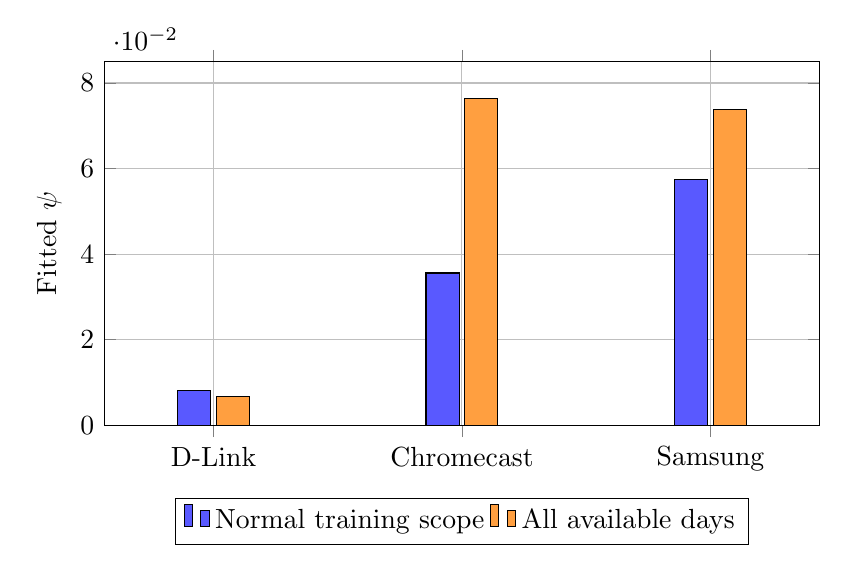
\begin{tikzpicture}
\begin{axis}[
  ybar,
  bar width=12pt,
  width=0.88\textwidth,
  height=6.2cm,
  ymin=0,
  ymax=0.085,
  ylabel={Fitted $\psi$},
  symbolic x coords={D-Link,Chromecast,Samsung},
  xtick=data,
  enlarge x limits=0.22,
  legend style={at={(0.5,-0.20)},anchor=north,legend columns=2},
  grid=major,
]
\addplot[fill=blue!65] coordinates {
  (D-Link,0.008182) (Chromecast,0.035589) (Samsung,0.057491)
};
\addlegendentry{Normal training scope}
\addplot[fill=orange!75] coordinates {
  (D-Link,0.006833) (Chromecast,0.076318) (Samsung,0.073784)
};
\addlegendentry{All available days}
\end{axis}
\end{tikzpicture}
\caption{The D-Link estimate remains low when all available days are combined.
The whole-dataset estimates rise for both labeled datasets, where the combined
scope includes temporal changes and attack-labelled windows.}
\label{fig:aggregate-psi}
\end{figure}

The comparison is especially relevant to LM. D-Link has the smallest fitted
\(\psi\), so it is closest to the Multinomial boundary and lies deepest in the
numerically delicate regime that motivated the LM calculation. Samsung has
the largest training \(\psi\), so at a fixed window total its fitted normal
model permits more compositional variation than the other two. Chromecast is
between them. This ordering concerns fitted dispersion; it does not by itself
rank anomaly-detection difficulty, because packet totals, category balance,
temporal changes, and attack types also differ.

\subsection{What the labels add to the comparison}

For Chromecast and Samsung, the labels allow the complete collection of rows
to be split into benign-labelled and attack-labelled subsets. Table
\ref{tab:label-split} is descriptive: each value is a new fit to the stated
subset. The attack fits use only 38 Chromecast windows and 82 Samsung windows,
and each subset combines several attack types, so these numbers should not be
treated as universal attack parameters.

\begin{table}[htbp]
\centering
\caption{Whole-dataset fits separated by the available window labels.}
\label{tab:label-split}
\begin{tabular}{lrrrr}
\toprule
Dataset & All rows & Benign-labelled & Attack-labelled & Attack windows \\
\midrule
D-Link camera & 0.006833 & -- & -- & -- \\
Chromecast & 0.076318 & 0.060307 & 0.577558 & 38 \\
Samsung Camera & 0.073784 & 0.023943 & 0.656396 & 82 \\
\bottomrule
\end{tabular}
\end{table}

For both labeled devices, the attack-only estimate is much larger than the
benign-only estimate. In these data, the attack windows therefore contain a
far less stable protocol composition under a single fitted
Dirichlet--multinomial model. The all-rows value lies between the two subset
fits and also reflects changes between days. D-Link has no corresponding
split, so its low all-days value cannot be used as evidence about attack
traffic; it is simply the value fitted to the unlabeled collection available
to the project.

\subsection{What the individual days reveal}

The aggregate values hide substantial day-to-day changes. Figure
\ref{fig:daily-psi} plots every daily fit on a logarithmic vertical scale. The
horizontal position is the chronological capture number within each device,
not a shared calendar date. Red triangles mark days containing at least one
attack-labelled window. The exact dates and values appear in
Table~\ref{tab:daily-psi}.

\begin{figure}[htbp]
\centering
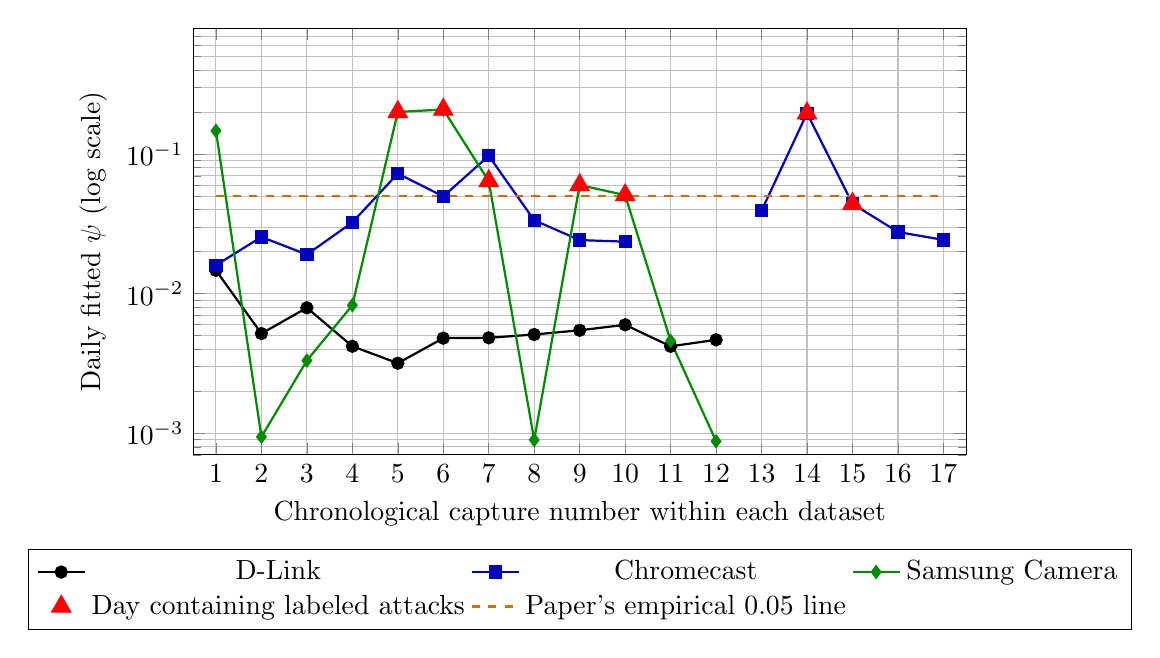
\begin{tikzpicture}
\begin{semilogyaxis}[
  width=0.94\textwidth,
  height=7.0cm,
  xmin=0.5,
  xmax=17.5,
  ymin=0.0007,
  ymax=0.8,
  xlabel={Chronological capture number within each dataset},
  ylabel={Daily fitted $\psi$ (log scale)},
  xtick={1,2,...,17},
  grid=both,
  unbounded coords=jump,
  legend style={at={(0.5,-0.22)},anchor=north,legend columns=3},
]
\addplot[black,mark=*,thick] coordinates {
  (1,0.014719) (2,0.005184) (3,0.007931) (4,0.004202)
  (5,0.003178) (6,0.004805) (7,0.004832) (8,0.005104)
  (9,0.005472) (10,0.005989) (11,0.004198) (12,0.004676)
};
\addlegendentry{D-Link}
\addplot[blue!75!black,mark=square*,thick] coordinates {
  (1,0.016012) (2,0.025523) (3,0.019097) (4,0.032473)
  (5,0.072661) (6,0.049859) (7,0.097399) (8,0.033622)
  (9,0.024242) (10,0.023627) (11,nan) (12,nan)
  (13,0.039374) (14,0.196667) (15,0.044145) (16,0.027706)
  (17,0.024312)
};
\addlegendentry{Chromecast}
\addplot[green!55!black,mark=diamond*,thick] coordinates {
  (1,0.147219) (2,0.000942) (3,0.003321) (4,0.008272)
  (5,0.201022) (6,0.209132) (7,0.064162) (8,0.000896)
  (9,0.060155) (10,0.050909) (11,0.004597) (12,0.000876)
};
\addlegendentry{Samsung Camera}
\addplot[red,only marks,mark=triangle*,mark size=4pt] coordinates {
  (14,0.196667) (15,0.044145)
  (5,0.201022) (6,0.209132) (7,0.064162)
  (9,0.060155) (10,0.050909)
};
\addlegendentry{Day containing labeled attacks}
\addplot[orange!85!black,dashed,thick,domain=1:17] {0.05};
\addlegendentry{Paper's empirical $0.05$ line}
\end{semilogyaxis}
\end{tikzpicture}
\caption{Daily reciprocal-concentration estimates. The logarithmic scale is
needed because the estimates span more than two orders of magnitude. A red
marker describes the complete day containing attacks, not an attack-only fit.}
\label{fig:daily-psi}
\end{figure}

\begin{table}[htbp]
\centering
\small
\caption{Daily fitted \(\psi\). ``Att.'' is the number of labeled attack
windows on that day; D-Link has no attack labels. A dash means that every
window was silent, so no protocol composition was available to fit.}
\label{tab:daily-psi}
\begin{tabular}{l r @{}c l r r l r r}
\toprule
\multicolumn{2}{c}{D-Link camera} &&
\multicolumn{3}{c}{Chromecast} &
\multicolumn{3}{c}{Samsung Camera} \\
\cmidrule(lr){1-2}\cmidrule(lr){4-6}\cmidrule(lr){7-9}
Date & \(\psi\) && Date & \(\psi\) & Att. & Date & \(\psi\) & Att. \\
\midrule
2020-10-08 & 0.014719 && 2018-10-10 & 0.016012 & 0 & 2018-05-28 & 0.147219 & 0 \\
2020-10-09 & 0.005184 && 2018-10-11 & 0.025523 & 0 & 2018-05-29 & 0.000942 & 0 \\
2020-10-10 & 0.007931 && 2018-10-12 & 0.019097 & 0 & 2018-05-30 & 0.003321 & 0 \\
2020-10-11 & 0.004202 && 2018-10-13 & 0.032473 & 0 & 2018-05-31 & 0.008272 & 0 \\
2020-10-12 & 0.003178 && 2018-10-14 & 0.072661 & 0 & 2018-06-01 & 0.201022 & 24 \\
2020-10-13 & 0.004805 && 2018-10-15 & 0.049859 & 0 & 2018-06-02 & 0.209132 & 42 \\
2020-10-14 & 0.004832 && 2018-10-16 & 0.097399 & 0 & 2018-06-03 & 0.064162 & 4 \\
2020-10-15 & 0.005104 && 2018-10-17 & 0.033622 & 0 & 2018-06-04 & 0.000896 & 0 \\
2020-10-16 & 0.005472 && 2018-10-18 & 0.024242 & 0 & 2018-06-05 & 0.060155 & 6 \\
2020-10-19 & 0.005989 && 2018-10-19 & 0.023627 & 0 & 2018-06-06 & 0.050909 & 6 \\
2020-10-21 & 0.004198 && 2018-10-20 & -- & 0 & 2018-06-07 & 0.004597 & 0 \\
2020-10-22 & 0.004676 && 2018-10-21 & -- & 0 & 2018-06-08 & 0.000876 & 0 \\
&&& 2018-10-22 & 0.039374 & 0 &&& \\
&&& 2018-10-23 & 0.196667 & 32 &&& \\
&&& 2018-10-25 & 0.044145 & 6 &&& \\
&&& 2018-10-26 & 0.027706 & 0 &&& \\
&&& 2018-10-27 & 0.024312 & 0 &&& \\
\bottomrule
\end{tabular}
\end{table}

The D-Link days form a comparatively narrow band: eleven of the twelve lie
between about 0.0032 and 0.0080, with October 8 at 0.0147. Chromecast varies
more, including two completely silent days for which \(\psi\) cannot be
estimated. Its largest daily value, 0.1967, occurs on October 23, which
contains 32 attack-labelled windows. Samsung changes most sharply: its daily
values range from about 0.00088 to 0.209, and its two largest values occur on
June 1 and June 2, which contain 24 and 42 attack-labelled windows.

The labels make those coincidences interpretable, but they do not prove that
every high daily value is caused by an attack. Chromecast October 16 reaches
0.0974 without a labeled attack, Samsung May 28 reaches 0.1472 without one,
and some attack-bearing days have much smaller values. A daily fit summarizes
all windows from that day, including benign traffic, attack traffic, changes
in activity, and differences in packet volume. It is therefore evidence about
the day's heterogeneity, not a detector output.

The main conclusion for the rest of this report is that rows carry real
information. The daily and label-separated fits change substantially when
different collections of windows are used. Pooling every row into one count
vector would retain the grand protocol totals but erase precisely the
window-to-window and day-to-day variation that the Dirichlet--multinomial model
is intended to represent in this project.

\section{Why the project evaluates windows separately with the LM backend}

\subsection{The project in a few paragraphs}

This project builds a small anomaly detector for Internet-of-Things network
traffic. It reads packet captures, assigns each supported packet to one of four
categories, and counts those packets over a configured time window. The
categories are TCP, UDP, SSDP, and ARP. SSDP is counted separately from ordinary
UDP, so each supported packet contributes to one category only.

The resulting count vector for one window is
\[
  \mathbf{x}_r =
  (x_{r,\mathrm{TCP}},x_{r,\mathrm{UDP}},
   x_{r,\mathrm{SSDP}},x_{r,\mathrm{ARP}}),
\]
where \(r\) identifies the window. A row is therefore not a category or a
packet: it is the complete four-category summary for one time window. During
training, the project collects many such rows from captures assigned to the
normal-training partition. Missing windows are left out because their traffic
is unknown; observed silent windows are retained as rows of zeros because they
are real observations of no captured packets.

The model learns a typical protocol mixture for one device and also allows
ordinary variation from window to window. It represents that mixture with a
Dirichlet--multinomial model whose parameters are collected in the vector
\(\boldsymbol{\alpha}\). The expected share of category \(k\) is
\(\alpha_k/\alpha_0\), where \(\alpha_0=\sum_k\alpha_k\). Once the model is
fitted, the detector can ask whether a new window looks plausible under the
device's learned normal behaviour.

\subsection{What the rows mean, and why keeping them matters}

The project treats each window as a separate observation from the same normal
device model. In practical terms, the model is meant to learn from a sequence of
window-sized snapshots, not just from one large bag of packets. Combining the
rows first would preserve the overall totals for TCP, UDP, SSDP, and ARP, but it
would erase which mixture occurred in which window. That distinction matters
when ordinary windows vary and when later decisions are made for individual
windows. This is the project's likelihood assumption; it does not by itself
prove that neighbouring windows are statistically independent. It says that,
for this fitting objective, each window contributes its own observation to the
shared device model.

Here is a small two-category example. The real project has four categories;
two are used here only to make the arithmetic easy to follow. Suppose two
windows contain
\[
  \mathbf{x}_1=(2,0), \qquad \mathbf{x}_2=(1,1).
\]
The first window contains only category A; the second contains both A and B.
If the rows are pooled, the only vector left is
\[
  \mathbf{x}_1+\mathbf{x}_2=(3,1).
\]
The pooled vector says that the dataset had three A counts and one B count. It
does not say that B was absent from the first window and present in the second.
For a model of window-level behaviour, that lost pattern is useful evidence
about how much windows vary.

The project therefore evaluates each row under the current model and adds the
log-likelihood contributions:
\[
  \ell_{\mathrm{rows}}(\boldsymbol{\alpha})
  = \ell(\mathbf{x}_1;\boldsymbol{\alpha})
    + \ell(\mathbf{x}_2;\boldsymbol{\alpha}).
\]
This is the usual way to combine log-likelihoods when treating observations
as separate samples: their probabilities multiply, and taking the logarithm
turns that product into a sum. The rows themselves are not added together.

The difference can be seen even with \(\boldsymbol{\alpha}=(1,1)\). The
parameter-dependent part of the Dirichlet--multinomial log-likelihood used by
the backends is
\[
  K(\mathbf{x};\boldsymbol{\alpha})
  = \log\Gamma(\alpha_0)-\log\Gamma(\alpha_0+N)
    + \sum_k\left[\log\Gamma(\alpha_k+x_k)
                   -\log\Gamma(\alpha_k)\right],
  \qquad N=\sum_k x_k.
\]
The backend leaves out the multinomial coefficient because it depends only on
the observed counts, not on alpha. For these rows, the calculations are:

\begin{center}
\begin{tabular}{p{0.33\linewidth}p{0.35\linewidth}r}
\toprule
Calculation & What is evaluated & Result \\
\midrule
Evaluate rows, then add & \(K((2,0);\alpha)+K((1,1);\alpha)\) & \(-2.89037\) \\
Add counts, then evaluate & \(K((3,1);\alpha)\) & \(-2.99573\) \\
\bottomrule
\end{tabular}
\end{center}

These are different because they answer different questions: the first
evaluates two observed windows, while the second evaluates one pooled count
vector. The example is not a claim that one number is inherently more
accurate; it illustrates that pooling changes the likelihood being
calculated. Leaving out the count-dependent coefficient does not affect which
alpha fits these same rows best; the scoring code adds that coefficient when
it needs the full single-window log-probability.

If the only scientific question were the device's total protocol composition
over a long period, pooling could be a reasonable summary. This detector also
models variation between windows and scores individual windows, so the project
keeps the windows separate for its likelihood objective. It still combines
their evidence into one dataset score by summing their likelihood values. That
final scalar is sufficient for fitting one shared alpha; the important part is
that each row affects the score through its own likelihood calculation before
the contributions are combined.

\subsection{How the professor's capsule handles the rows}

The original capsule does not discard the rows from all of its fitting logic.
Its Minka fixed-point update reads the original matrix \texttt{D\_counts} and
loops over its rows when it forms the update. For a given category, it adds the
row-specific digamma contributions; it also uses each row's total count in the
concentration update. Thus the update step is based on the individual rows.

The difference is in the likelihood calculation used by the original
LM-wrapped fitting path. Before the LM likelihood is called, the helper
\texttt{find\_X(D\_counts)} adds each category's counts down the rows. For the
example above, it turns the two rows into the single vector \((3,1)\). The
fitting function then derives the category probabilities and dispersion
parameter from its current alpha vector and calls the scalar C function
\texttt{loggamma\_LM} once for the old alpha and once for the candidate alpha.
Those calls evaluate the likelihood of the pooled count vector. Their
difference is used in the capsule's stopping check.

The main functions to recognize in the original source are:

\begin{center}
\begin{tabular}{>{\ttfamily}p{0.34\linewidth}p{0.57\linewidth}}
\toprule
Function & Role in the original fitting path \\
\midrule
\texttt{load\_dataset\_from\_file} & Reads the count matrix and prepares it for fitting. \\
\texttt{find\_X} & Sums each category column across all rows, producing one pooled count vector. \\
\texttt{minka\_procedure\_LM\_c\_wrapped\_mode} & Updates alpha from the separate rows, then compares LM likelihoods for the pooled vector to decide when to stop. \\
\texttt{loggamma\_LM} & Scalar native entry point used by that fitting function for one count vector and one alpha setting. \\
\texttt{logL\_diretta\_global} & Evaluates the scalar vector's Dirichlet--multinomial log-likelihood kernel using the LM calculation. \\
\bottomrule
\end{tabular}
\end{center}

The capsule's likelihood helper \texttt{LM\_logL\_dataset} also takes a single
count vector \texttt{X}; it forms one total count and combines the category
terms for that vector. In the C-wrapped fitting route, the corresponding
single-vector call is \texttt{loggamma\_LM}. The word ``dataset'' in the helper
name can be misleading here: the likelihood call receives a category-total
vector, not the original matrix of separate windows.

So, if the question is whether the professor's LM likelihood call sums the
individual row likelihoods, the answer for this original fitting path is no.
It evaluates one likelihood for the column-summed vector. If the question is
whether the professor's entire estimator uses the rows, the answer is yes: the
Minka updates do. The project changed the likelihood objective used with those
updates so that it also represents the rows separately.

\subsection{How the project calls the LM code}

The project has its own estimator. Its Minka fixed-point updates are implemented
in Python in \texttt{DirichletMultinomialEstimator}; they use the rows of the
training matrix. The estimator asks a common likelihood interface to evaluate
the current and updated alpha values. That interface can use either SciPy or
the LM backend.

With the LM backend selected, the call travels through
\texttt{LmLogLikelihood.calculate}, then the Python-to-C bridge
\texttt{NativeLmKernel.calculate}, and finally into the native matrix function
\texttt{loggamma\_LM\_matrix}. The original scalar LM calculation remains the
numerical engine for an individual row. The project-side matrix function
accepts all rows, evaluates each one with the same alpha parameters, and returns
the sum of their likelihood-kernel values.

In outline, the project's calculation is:
\begin{verbatim}
total = 0
for each window row:
    total += LM_likelihood_for_one_row(row, alpha)
return total
\end{verbatim}
The important detail is the order: evaluate a row first, then add the resulting
likelihood value. It does not add the count rows first.

\subsection{Why the project-side LM integration was adapted}

The professor's scalar LM entry point was designed to calculate the likelihood
for one count vector at a time. The project's estimator supplies a matrix
because its fitting objective treats each time window as its own observation.
The first project-side adaptation added a matrix entry point that bridges those
two shapes: it accepts the matrix, sends each row through the existing scalar
LM calculation, and adds the returned values. It also checks that the inputs
and numerical results are valid and cleans up the native workspace on success
or failure. The original files in \texttt{lm-algorithm/code/} were left
unchanged; the application-facing changes are in the project's copy under
\texttt{src/lm\_idnet/algorithms/native/}.

That first version repeated setup for every row. The LM routine needed values
derived from alpha and the requested precision, and it searched for an
Euler--Maclaurin expansion order and a horizontal shift that met the requested
error bound. Within one matrix call, those setup inputs are the same for every
row. Repeating the setup did not make the rows more accurate; it did the same
work again.

The later optimization moved the shared setup before the row loop. It prepares
the native workspace and selects the expansion order and horizontal shift once,
then evaluates each row separately using that shared setup, adds the row
results, and releases the workspace. Checks that depend on a row's counts
remain inside the loop. In outline:
\begin{verbatim}
prepare LM settings for this alpha and precision
total = 0
for each window row:
    check this row
    total += LM_likelihood_for_one_row_using_prepared_settings(row)
release LM workspace
return total
\end{verbatim}

This optimization does not pool rows. It also does not change the LM
approximation, its error-control rules, Minka's update, or the row-wise
likelihood being computed. The change record reports that the old and optimized
project libraries returned identical values across 1,000 tested matrices. In
that controlled comparison, the 846-row likelihood call became 51.5\% faster.
Those are results for the project's matrix calculation and workload; they do
not establish that every LM operation is faster than SciPy.

\subsection{A concise explanation for the meeting}

The project represents a device's traffic as one four-category count row per
time window, because it needs to model normal variation between windows and
score windows individually. The professor's original LM-wrapped fit also uses
the individual rows in the Minka update, but it sums the count columns before
calling its scalar LM likelihood for the stopping comparison. The project
instead passes the rows to its LM backend, calculates each row's likelihood
contribution, and sums those values, which is the dataset log-likelihood for
separate observations. The project-side LM adapter was added to make the
professor's one-vector numerical routine accept that matrix calculation; its
subsequent optimization reuses alpha- and precision-dependent setup across the
rows. It preserves the same row-wise result while avoiding repeated setup.

\subsection{The other native changes, in one minute}

The row-wise interface and its setup optimization are the changes that need
the detailed explanation above. The remaining changes to the project copy of
the professor's native code can be summarized briefly:

\begin{itemize}

\item \textbf{Exact zero-count handling.} A zero packet count contributes
exactly zero to the paired log-gamma difference, so the native function now
returns that identity directly. This matters because an otherwise valid
window can have zero packets in one category, and a silent window has zero in
every category.

\item \textbf{Reliable coefficient-table loading.} The two tables needed by
the likelihood path are now loaded from explicit paths supplied by the Python
adapter. Both files are validated before the active tables are replaced, and
failure is returned to the caller instead of depending on the process's
current directory or terminating the application.

\item \textbf{Explicit native-memory ownership.} Parameter arrays and the
temporary error-search workspace are checked after allocation and released on
success and failure paths. This prevents repeated likelihood calls during
fitting from accumulating leaked native memory.

\item \textbf{Controlled library rebuild.} The modified source was rebuilt
with the project's existing compiler image and optimization flags, then
checked against the source and exercised through the Python adapter. This step
does not change the mathematics; it ensures that the shared library actually
contains the reviewed source changes.

\end{itemize}

\section{What was timed and what the runtime numbers mean}

Runtime claims are meaningful only when the timed operation is named. This
project contains several operations that all involve a likelihood, but they
answer different questions and have very different costs. In particular, the
reported ``complete model fit'' is not the complete command-line pipeline, and
the time printed by the professor's original capsule is not the complete fit
wall time.

The broad application flow is
\[
\boxed{
\begin{gathered}
\text{packet preprocessing}
\longrightarrow \text{load processed rows}
\longrightarrow \text{fit }\boldsymbol{\alpha}
\longrightarrow \text{save model}\,,\\
\text{load calibration rows}
\longrightarrow \text{calculate calibration scores}
\longrightarrow \text{choose threshold}\,,\\
\text{load later rows}
\longrightarrow \text{score each window}
\longrightarrow \text{record decisions and evaluate labels}.
\end{gathered}}
\]

Packet preprocessing is intentionally outside the runtime analysis. None of
the results below includes reading PCAP files, classifying packets, or building
ten-minute windows. More importantly, no single reported number times every
remaining box in this diagram. The benchmark separates model fitting, one
training-matrix likelihood call, and one single-window score so that the source
of a speed difference can be understood.

\subsection{The four timing scopes that must not be confused}

Table~\ref{tab:timing-boundaries} states where each timer starts and stops.
The first three scopes belong to the production benchmark. The last is the
timer used by the professor's original fitting code.

\begin{table}[htbp]
\centering
\small
\caption{Meaning of each runtime measurement.}
\label{tab:timing-boundaries}
\begin{tabular}{p{0.18\textwidth}p{0.35\textwidth}p{0.36\textwidth}}
\toprule
Measurement & Included & Excluded \\
\midrule
Complete model fit & Initial alpha construction; the initial matrix
likelihood; every row-wise Minka digamma update; one matrix likelihood after
each update; convergence checks; construction of the fit result. & PCAP
preprocessing; loading processed JSON; construction of the backend and loading
its coefficient tables; saving the model; calibration; later scoring;
evaluation. \\
\addlinespace
Training-matrix likelihood & One call to
\texttt{backend.calculate(training.counts, reference\_alpha)}. It includes
Python validation, conversion from alpha to probabilities and \(\psi\), the
backend calculation, and return to Python. & Alpha initialization; Minka
updates; repeated convergence iterations; the count-only multinomial
coefficient; file input and output. \\
\addlinespace
Single-window score & The complete log-probability for one representative
non-silent window: its multinomial coefficient plus one one-row backend
likelihood, followed by the configured raw-score return. & Loading the window;
threshold comparison; event construction; writing output; calibration and
label evaluation. \\
\addlinespace
Original capsule's printed time & The accumulated duration of two likelihood
calls in every Minka iteration: one at the old alpha and one at the candidate
alpha. & The Minka digamma update, alpha and probability preparation, dataset
loading, initialization outside those calls, forecasting, and all other wall
time. \\
\bottomrule
\end{tabular}
\end{table}

The benchmark command does run isolated training, calibration, and scoring
paths for both backends so that their models, thresholds, scores, and decisions
can be compared. That execution is a correctness check. Its combined wall time
is not reported as a pipeline benchmark. Therefore the phrase ``complete model
fit'' should be used instead of ``complete pipeline'' when presenting the
numbers below.

\subsection{Initial likelihood, iterative likelihood, and scoring likelihood}

The word ``likelihood'' appears at three different moments in the project, so
it is useful to follow one fit from the beginning.

First, the project creates an initial alpha vector from the category totals and
the configured initial concentration. The likelihood does not calculate this
alpha vector. After alpha has been initialized, the estimator calculates one
initial likelihood and stores it as the baseline for convergence.

Next, every Minka iteration calculates a new alpha vector from digamma
differences over the individual rows. LM and SciPy do not perform this update;
both versions use the same SciPy digamma calculation. The selected backend then
evaluates the row-wise likelihood at the new alpha. The estimator compares
that value with the likelihood retained from the preceding step. If their
absolute difference is below the tolerance, fitting stops. Otherwise the new
value becomes the previous value for the next iteration.

In simplified form, the production estimator does this:
\begin{verbatim}
alpha = initialize_alpha(training_rows)
previous = matrix_likelihood(training_rows, alpha)  # one initial call

for each Minka iteration:
    alpha = digamma_fixed_point_update(training_rows, alpha)
    current = matrix_likelihood(training_rows, alpha)  # one call
    if abs(current - previous) < tolerance:
        stop
    previous = current
\end{verbatim}

Thus a fit lasting \(I\) iterations performs \(I+1\) matrix-likelihood calls:
one before the loop and one after each update. The likelihood guides the
stopping decision; the digamma formula produces alpha.

Much later, during anomaly detection, the fitted alpha is fixed. A new window
is assigned the full log-probability
\[
  \log P(\mathbf{x}\mid\boldsymbol{\alpha})
  = \log\frac{N!}{\prod_k x_k!}
    + K(\mathbf{x};\boldsymbol{\alpha}).
\]
Here \(K\) is the backend likelihood kernel explained in Section~I. The
count-only multinomial coefficient is added for scoring because different
windows are being compared. This scoring calculation does not update alpha and
does not run Minka iterations.

The stored initial and final likelihoods are numerical values, not timing
measurements. Table~\ref{tab:fit-workloads} shows the current LM fits and also
explains why absolute fit times cannot be compared across devices without
considering both matrix size and iteration count.

\begin{table}[htbp]
\centering
\small
\caption{Production training workloads and stored LM convergence values.}
\label{tab:fit-workloads}
\begin{tabular}{lrrrr}
\toprule
Dataset & Matrix & Iterations & Initial likelihood & Final likelihood \\
\midrule
D-Link camera & \(846\times4\) & 1,882 & $-477{,}950.796$ & $-476{,}052.589$ \\
Chromecast & \(867\times4\) & 1,950 & $-1{,}464{,}261.145$ & $-1{,}462{,}542.173$ \\
Samsung Camera & \(432\times4\) & 580 & $-191{,}965.774$ & $-191{,}562.039$ \\
\bottomrule
\end{tabular}
\end{table}

These likelihood values are sums of the parameter-dependent kernel across the
training rows. Their magnitudes depend on the data and row counts, so they
should not be compared as if a less negative value identified the better
device model. Within one fit, the change is used only to decide when the alpha
sequence has settled.

\subsection{How the production benchmark was measured}

The production comparison gives LM and SciPy the same processed count matrix,
the same estimator settings, and the same scoring workload. Backend objects are
constructed before the timers start, so LM's one-time shared-library load and
coefficient-table initialization are not charged to a likelihood call or fit.
This is appropriate for a service that initializes its backend once and then
uses it repeatedly, but it should be stated explicitly.

Complete fitting is measured five times per backend and reported as the median.
The isolated likelihood and score operations are warmed once, then measured in
five batches. Each likelihood batch contains 200 calls and each score batch
contains 1,000 calls; the reported value is the median per-call duration. The
standalone likelihood and score comparisons use the alpha fitted by the SciPy
training run for both backends. This prevents a tiny backend-dependent alpha
difference from changing the timed workload.

The cross-dataset measurements in the full project report were collected on
9 September 2026 on the same x86-64 development environment, using Python
3.12.14, NumPy 2.5.1, and SciPy 1.18.0. They are development-machine results,
not measurements from an edge device, and normal system timing noise still
applies.

\subsection{Current production results: LM compared with SciPy}

Figure~\ref{fig:section-two-runtime} and
Table~\ref{tab:section-two-runtime} show the same three operations. Lower is
better. Within each dataset, the LM/SciPy ratio is the useful comparison:
values above one mean LM took longer and values below one mean LM took less
time.

\begin{figure}[htbp]
\centering
\begin{tikzpicture}
\begin{groupplot}[
  group style={group size=3 by 1,horizontal sep=0.8cm},
  ybar,
  bar width=5pt,
  width=0.29\textwidth,
  height=0.31\textwidth,
  ymin=0,
  symbolic x coords={dlink,chromecast,samsung},
  xtick=data,
  xticklabels={D-Link,Chromecast,Samsung},
  x tick label style={font=\scriptsize,rotate=28,anchor=east},
  y tick label style={font=\scriptsize},
  grid=major,
  grid style={gray!20},
  enlarge x limits=0.22,
  title style={font=\small\bfseries},
  legend style={font=\small,draw=none,at={(1.72,-0.36)},anchor=north,
    legend columns=2},
]
\nextgroupplot[title={Complete model fit},ylabel={Time (ms)},ymax=285]
\addplot[fill=blue!65] coordinates {
  (dlink,191.04) (chromecast,254.17) (samsung,42.46)
};
\addlegendentry{LM}
\addplot[fill=green!55] coordinates {
  (dlink,180.59) (chromecast,194.40) (samsung,34.47)
};
\addlegendentry{SciPy}

\nextgroupplot[title={Training likelihood},ylabel={Time ($\mu$s)},ymax=95]
\addplot[fill=blue!65] coordinates {
  (dlink,55.02) (chromecast,84.69) (samsung,45.69)
};
\addplot[fill=green!55] coordinates {
  (dlink,49.79) (chromecast,52.12) (samsung,31.57)
};

\nextgroupplot[title={Single-window score},ylabel={Time ($\mu$s)},ymax=15]
\addplot[fill=blue!65] coordinates {
  (dlink,12.00) (chromecast,12.22) (samsung,12.18)
};
\addplot[fill=green!55] coordinates {
  (dlink,13.18) (chromecast,13.22) (samsung,13.20)
};
\end{groupplot}
\end{tikzpicture}
\caption{Median runtime for the three separately timed production operations.
The fit uses an already loaded matrix, the training likelihood is one matrix
call at fixed alpha, and the score is one complete single-window score.}
\label{fig:section-two-runtime}
\end{figure}

\begin{table}[htbp]
\centering
\small
\caption{Production LM/SciPy runtime comparison. A positive difference means
LM was slower; a negative difference means LM was faster.}
\label{tab:section-two-runtime}
\begin{tabular}{llrrrr}
\toprule
Operation & Dataset & SciPy & LM & LM/SciPy & Difference \\
\midrule
Complete fit & D-Link & 180.59 ms & 191.04 ms & 1.058 & $+5.8\%$ \\
& Chromecast & 194.40 ms & 254.17 ms & 1.307 & $+30.7\%$ \\
& Samsung & 34.47 ms & 42.46 ms & 1.232 & $+23.2\%$ \\
\addlinespace
Matrix likelihood & D-Link & 49.79 $\mu$s & 55.02 $\mu$s & 1.105 & $+10.5\%$ \\
& Chromecast & 52.12 $\mu$s & 84.69 $\mu$s & 1.625 & $+62.5\%$ \\
& Samsung & 31.57 $\mu$s & 45.69 $\mu$s & 1.447 & $+44.7\%$ \\
\addlinespace
Single score & D-Link & 13.18 $\mu$s & 12.00 $\mu$s & 0.910 & $-9.0\%$ \\
& Chromecast & 13.22 $\mu$s & 12.22 $\mu$s & 0.924 & $-7.6\%$ \\
& Samsung & 13.20 $\mu$s & 12.18 $\mu$s & 0.923 & $-7.7\%$ \\
\bottomrule
\end{tabular}
\end{table}

The current LM backend is slower than SciPy for the complete row-wise training
likelihood on every dataset in this run. It is correspondingly slower for the
complete fit. The size of the full-fit difference does not exactly equal the
matrix-likelihood difference because the fit also spends time in alpha
initialization and in the shared SciPy digamma updates. Samsung is fastest in
absolute terms because it has only 432 training rows and reaches convergence in
about 580 iterations; this does not mean its individual likelihood operation is
the fastest relative to SciPy.

The result reverses for single-window scoring. LM takes about 12.0--12.2
microseconds and SciPy about 13.2 microseconds, making LM roughly 8--9 percent
faster on this workload. A score calls the backend on only one row, where LM's
native evaluation is competitive and there is no large matrix traversal. This
is the operation closest to the detector's repeated online work, although the
measurement still excludes packet capture, window construction, threshold
comparison, and output.

An independently stored D-Link run produced 0.19297 seconds versus 0.18129
seconds for the complete fit, 55.46 versus 49.96 microseconds for the matrix
likelihood, and 12.04 versus 13.39 microseconds for a score. These values differ
slightly from the cross-dataset run because they were recorded in a separate
timing session, but they support the same conclusion: current LM is close to
SciPy for this complete fit, slower for the large matrix call, and faster for
one-window scoring. The independent D-Link fit is 6.4 percent slower, which is
inside the 10 percent ``no significant speed difference'' criterion used in
the professor's IoT study. Chromecast and Samsung exceed that margin in the
cross-dataset production run, so the criterion should not be generalized to
all three fits.

\subsection{What the optimization changed}

Three code states appear in the discussion, and their names should be kept
precise. The reference files under \texttt{lm-algorithm/code/} remain
untouched; all application changes were made in the project's runtime copy.

\begin{table}[htbp]
\centering
\small
\caption{The three LM implementations referred to in the runtime discussion.}
\label{tab:three-lm-states}
\begin{tabular}{p{0.20\textwidth}p{0.31\textwidth}p{0.37\textwidth}}
\toprule
Code state & Likelihood semantics & Execution pattern \\
\midrule
Original professor capsule & Sum the count rows first and evaluate one pooled
vector for convergence. & Scalar LM entry point; old and candidate likelihood
both recalculated each iteration; printed time contains only those calls. \\
\addlinespace
Earlier project adapter & Evaluate every row independently and then sum the
likelihood values. & Matrix wrapper calls the professor's complete scalar setup
and evaluation sequence for every row. \\
\addlinespace
Current project adapter & The same row-wise likelihood as the earlier project
adapter. & Matrix wrapper performs common setup once, then retains separate
validation and likelihood evaluation for every row. \\
\bottomrule
\end{tabular}
\end{table}

The most important before-and-after comparison is between two versions of the
project's row-wise LM adapter. It is not a comparison between the untouched
professor capsule and the production detector. Both versions below calculate
the same row-wise matrix likelihood. The earlier adapter safely called the
professor's single-vector setup and evaluation sequence once per row. The
optimized adapter prepares the alpha- and precision-dependent state once,
retains all row-specific checks and evaluations, and releases the workspace at
the matrix boundary.

\begin{table}[htbp]
\centering
\small
\caption{Controlled D-Link before-and-after result for the row-wise project
implementation.}
\label{tab:optimization-effect}
\resizebox{\textwidth}{!}{%
\begin{tabular}{lrrrr}
\toprule
Operation & SciPy & Earlier project LM & Current project LM & LM reduction \\
\midrule
\(846\times4\) likelihood & 49.96 $\mu$s & 114.68 $\mu$s & 55.58 $\mu$s & 51.5\% \\
Complete model fit & 0.18129 s & 0.30410 s & 0.19486 s & 35.9\% \\
\bottomrule
\end{tabular}
}
\end{table}

Before this optimization, the LM matrix call was about 2.30 times the SciPy
time and the complete fit was about 1.68 times the SciPy time. Afterwards the
ratios were about 1.11 and 1.07. The likelihood speedup is larger than the fit
speedup because only the LM likelihood portion was changed; Minka's digamma
work remained the same.

The old and optimized project libraries produced bit-for-bit identical results
over 1,000 deterministic stress matrices. Therefore the reduction measures the
removal of repeated setup, not a relaxation of precision, a change in the
row-wise objective, or fewer Minka iterations. This is the strongest runtime
improvement attributable directly to the native-code modification.

\subsection{Why the original professor timing gives a different answer}

The original capsule uses a different calling pattern. Its Minka update still
reads every row, but it first sums the rows into one count vector for the
convergence likelihood. During each iteration it calculates the likelihood at
both the old and candidate alpha values:
\begin{verbatim}
for each Minka iteration:
    candidate_alpha = digamma_fixed_point_update(all_rows, old_alpha)
    start timer
    old_value = likelihood(sum(all_rows), old_alpha)
    stop timer
    start timer
    new_value = likelihood(sum(all_rows), candidate_alpha)
    stop timer
    add both durations to reported likelihood time
\end{verbatim}

The old likelihood in one iteration is normally the new likelihood from the
preceding iteration, but the capsule calculates it again. Its printed
\texttt{time} is the sum of these two timed calls, not the elapsed time from the
start to the end of fitting. By comparison, the production estimator retains
the preceding value and performs one new row-wise likelihood call per
iteration. The original capsule also uses a moment-based initial alpha and
changes any row containing a zero by adding one to all its categories. The
production estimator starts from observed category totals at a configured
concentration and accepts zero counts directly. Finally, the capsule expresses
much of the update as Python loops, whereas the production estimator uses
NumPy array operations. The two programs therefore differ in row semantics,
number of likelihood calls, initialization, zero handling, implementation of
the update, and timer scope. Their raw printed times cannot be placed in one
table as though they measured the same operation.

To make the professor-style architecture measurable, the project reproduced
that calling pattern on deterministic samples from seven D-Link days. The
experiment records both the accumulated likelihood-call time, matching the
meaning of the capsule's timer, and a separate wall timer around the iteration
loop. That wall timer starts after the rows have been aggregated and the
moment-based initial alpha has been constructed. It includes the digamma
updates, both likelihood calls, convergence checks, and loop overhead, but not
data loading or those two setup steps. Each percentage below compares LM and
SciPy within that same aggregate architecture. The reproduction uses the
project's vectorized update and backend interfaces, so it reproduces the
professor-style statistical and calling structure rather than timing the
untouched capsule line for line.

\begin{table}[htbp]
\centering
\small
\caption{Professor-style aggregate experiment. Each time is the mean total for
fitting seven daily samples across three deterministic repeats.}
\label{tab:professor-style-times}
\resizebox{\textwidth}{!}{%
\begin{tabular}{rrrrrrrr}
\toprule
Sample & Converged & \multicolumn{3}{c}{Likelihood-call time} &
\multicolumn{3}{c}{Iteration-loop wall time} \\
\cmidrule(lr){3-5}\cmidrule(lr){6-8}
& & SciPy & LM & Reduction & SciPy & LM & Reduction \\
\midrule
10\% & 17/21 & 3.5746 s & 3.1396 s & 12.2\% & 4.8933 s & 4.4593 s & 8.9\% \\
15\% & 20/21 & 1.9094 s & 1.6766 s & 12.2\% & 2.6517 s & 2.4187 s & 8.8\% \\
20\% & 21/21 & 1.6485 s & 1.4447 s & 12.4\% & 2.3125 s & 2.1064 s & 8.9\% \\
25\% & 21/21 & 0.9779 s & 0.8599 s & 12.1\% & 1.3957 s & 1.2799 s & 8.3\% \\
\midrule
All 84 fits & 79/84 & 24.3311 s & 21.3625 s & 12.2\% & 33.7594 s & 30.7930 s & 8.8\% \\
\bottomrule
\end{tabular}
}
\end{table}

In that experiment, LM is faster: it reduces the time spent in aggregate
likelihood calls by 12.2 percent and the iteration-loop wall time by 8.8 percent.
The same five samples fail to converge with both backends, so the difference is
not created by one backend abandoning extra fits. On the complete
\(846\times4\) D-Link matrix, one pooled-vector call takes 8.44 microseconds
with LM and 9.72 microseconds with SciPy, and a literal professor-style fit
loop takes 0.15909 seconds with LM versus 0.16425 seconds with SciPy.

Those results do reproduce the runtime advantage of LM under the professor's
aggregate calling pattern. They do not contradict the production results.
Pooling changes an 846-row likelihood into one vector evaluation and therefore
removes the workload on which SciPy's vectorization is strongest. It also
changes the convergence objective, as explained in Section~I. The aggregate
experiment is evidence about the reference architecture; the row-wise
benchmark is evidence about the anomaly detector actually implemented here.

\subsection{Runtime must be read together with numerical agreement}

A faster result is useful only if the two backends still implement the same
calculation closely enough for the application. In the stored D-Link production
benchmark, the maximum relative difference between fitted alpha values was
\(3.86\times10^{-7}\), the maximum absolute score difference was
\(1.09\times10^{-5}\), and the threshold difference was
\(2.89\times10^{-6}\). Both backends flagged the same three windows, with zero
decision mismatches across 270 development windows. D-Link is unlabeled, so
this demonstrates backend agreement rather than detection accuracy.

The same practical check was made when the three versioned device
configurations were regenerated with LM after previously using SciPy. Across
their 1,300 development windows, the largest relative alpha difference was
\(1.71\times10^{-6}\), the largest absolute score difference was
\(1.78\times10^{-4}\), and every anomaly decision was retained: 3 D-Link, 17
Chromecast, and 52 Samsung Camera windows were flagged by both sets of
artifacts. For Chromecast and Samsung those counts can be evaluated against
labels elsewhere in the project; here they establish only that changing the
numerical backend did not change a decision.

The current D-Link fit is not numerically extreme. At its concentration of
about 122.22, or \(\psi\approx8.18\times10^{-3}\), comparison with
100-decimal-digit arithmetic gave an absolute error of
\(3.07\times10^{-10}\) for SciPy and \(3.91\times10^{-10}\) for LM. Both are
already highly accurate. The reason to retain LM becomes clearer much closer
to the Multinomial boundary:

\begin{table}[htbp]
\centering
\caption{Absolute error of one aggregate likelihood against high-precision
arithmetic as concentration increases and \(\psi\) decreases.}
\label{tab:low-psi-accuracy}
\begin{tabular}{rrrr}
\toprule
Concentration & \(\psi\) & SciPy error & LM error \\
\midrule
122.22 & \(8.18\times10^{-3}\) & \(3.07\times10^{-10}\) & \(3.91\times10^{-10}\) \\
\(10^8\) & \(10^{-8}\) & \(2.50\times10^{-7}\) & \(1.50\times10^{-8}\) \\
\(10^{10}\) & \(10^{-10}\) & \(2.83\times10^{-5}\) & \(5.65\times10^{-8}\) \\
\(10^{12}\) & \(10^{-12}\) & \(2.02\times10^{-3}\) & \(5.58\times10^{-5}\) \\
\(10^{14}\) & \(10^{-14}\) & \(3.37\times10^{-1}\) & \(1.03\times10^{-3}\) \\
\bottomrule
\end{tabular}
\end{table}

This table explains the actual tradeoff. On the current datasets, SciPy is
already accurate and often faster for fitting a complete matrix. LM provides
much better protection against cancellation at extremely small \(\psi\), and
the optimized native path is slightly faster for the repeated one-window score
operation measured here.

\subsection{The runtime conclusion to present}

The clearest account for the meeting is the following. Preprocessing was
deliberately excluded. The project did not report one end-to-end time for
loading, fitting, calibration, scoring, and evaluation. It separately measured
the estimator fit on an already loaded training matrix, one row-wise
training-matrix likelihood call at fixed fitted alpha, and one full anomaly
score for a representative window.

The earlier row-wise LM adapter was slow because it repeated invariant native
setup for every row. Reusing that setup cut its D-Link matrix-likelihood time
by 51.5 percent and its complete-fit time by 35.9 percent without changing any
result. After that optimization, LM is close to SciPy on the D-Link complete
fit, slower on the three large matrix likelihoods and complete fits in the
cross-dataset benchmark, and about 8--9 percent faster for one-window scoring.

The professor-style aggregate experiment remains a separate and valid result.
Under that architecture, LM reduces accumulated likelihood time by 12.2
percent and iteration-loop wall time by 8.8 percent. It cannot be used as the
runtime of the production row-wise detector because it pools the rows, performs
two likelihood calls per iteration, and times a different calculation. The
defensible claim is therefore conditional: the native optimization materially
improved the project integration, and LM's speed relative to SciPy depends on
the operation and calling architecture being measured.

\section*{Source trail}

The dispersion comparison uses the processed windows under
\texttt{data/processed/}, the daily fits in each dataset's
\texttt{reports/.../capture\_statistics.json}, the stored training models
under \texttt{artifacts/}, and the UNSW window annotations under
\texttt{data/labels/}. Aggregate, benign-only, and attack-only values were
fitted with the same row-wise LM estimator and settings used by the project;
labels were joined to processed rows by window start time. Pearson ratios use
the common-probability Multinomial calculation stated in Section~0.

The production timing definitions follow
\texttt{src/lm\_idnet/evaluation/benchmark\_stage.py}, with the D-Link audit
record in \texttt{reports/D-LinkDayCam5/lm\_backend\_benchmark.json}. The
three-dataset measurements are recorded in
\texttt{docs/lm\_idnet\_full\_project\_report.tex}. The controlled native
before-and-after figures come from
\texttt{docs/lm\_backend\_change\_record.tex}. The aggregate architecture,
including its separate likelihood and wall timers, is implemented in
\texttt{scripts/lm\_professor\_experiment.py} and recorded in
\texttt{reports/D-LinkDayCam5/lm\_professor\_experiment.json} and
\texttt{docs/lm\_professor\_architecture\_experiment\_report.md}.

The descriptions of the adaptations follow
\texttt{docs/lm\_backend\_change\_record.tex}. The original capsule functions
described above are in \texttt{lm-algorithm/code/LogL-global-v5.py} and its
native files, especially \texttt{LM\_time\_lib.c}. The project path is visible
in \texttt{src/lm\_idnet/models/modeling\_stage.py},
\texttt{src/lm\_idnet/algorithms/dirichlet.py},
\texttt{src/lm\_idnet/algorithms/log\_likelihood.py},
\texttt{src/lm\_idnet/algorithms/lm\_native.py}, and the native LM source
under \texttt{src/lm\_idnet/algorithms/native/}.

\end{document}
